%%%%%%%%%%%%%%%%%%%% author.tex %%%%%%%%%%%%%%%%%%%%%%%%%%%%%%%%%%%
%
% sample root file for your "contribution" to a proceedings volume
%
% Use this file as a template for your own input.
%
%%%%%%%%%%%%%%%% Springer %%%%%%%%%%%%%%%%%%%%%%%%%%%%%%%%%%


\documentclass{svproc}
%
% RECOMMENDED %%%%%%%%%%%%%%%%%%%%%%%%%%%%%%%%%%%%%%%%%%%%%%%%%%%
%
\usepackage{graphicx}
\usepackage{marvosym}

% to typeset URLs, URIs, and DOIs
\usepackage{url}
\usepackage{hyperref}
\def\UrlFont{\rmfamily}

\def\orcidID#1{\unskip$^{[#1]}$}
\def\letter{$^{\textrm{(\Letter)}}$}

\begin{document}
\mainmatter              % start of a contribution
%
\title{Parallel Computing in Tikhonov Regularization Method for Solving the Inverse Problem of Chemical Kinetics}

%Parallel computing in Tikhonov regularization method for solving the inverse problem of chemical kinetics

%Solving the Regularized Inverse Problem of Chemical Kinetics Using the Parallel Optimization Algorithm


%
\titlerunning{Parallel Computing}  % abbreviated title (for running head)
%                                     also used for the TOC unless
%                                     \toctitle is used
%
\author{Konstantin Barkalov\inst{1}\letter\orcidID{0000-0001-5273-2471} \and Marina Usova\inst{1}\orcidID{0000-0002-0722-6884} \and Leniza Enikeeva\inst{2}\letter\orcidID{0000-0003-4219-4870} \and Dmitry Dubovsev\inst{3} \and Irek Gubaydullin\inst{2,3}}

%
\authorrunning{K. Barkalov et al.} % abbreviated author list (for running head)
%
%%%% list of authors for the TOC (use if author list has to be modified)
%\tocauthor{Ivar Ekeland and Kim~B.~Bruce, and Roger Temam}
%
\institute{Lobachevsky State University of Nizhny Novgorod, Nizhny Novgorod, Russia \\
	\email{konstantin.barkalov@itmm.unn.ru}
	\and
	Ufa State Petroleum Technological University, Ufa, Russia \\
	\email{leniza.enikeeva@yandex.ru} \\
        \and
        Institute of Petrochemistry and Catalysis – Subdivision of the Ufa Federal Research Centre of RAS, Ufa, Russia
}

	
\maketitle              % typeset the title of the contribution

\begin{abstract}
% Проверьте первое предложение - мой вариант ниже
% The authors investigates the advantages and disadvantages of the products refining processes used in the gasoline production. 
The authors investigates the advantages and disadvantages of the products refining processes used in the gasoline production. As one of the ways to solve the problem of environmental friendliness of motor fuel, it is proposed to consider increasing the practice of involving alkylate in compounding and improving its quality. The work describes the scheme of chemical transformations of the sulfuric acid alkylation process, taking into account the target reactions and side effects. Based on the studied chemistry of the reactions, the authors pose the inverse problem of chemical kinetics and consider the regularization method for its solution. 
The global optimization problem, which corresponds to the regularized inverse problem, was solved using a parallel optimization algorithm.
The results of a computational experiment on a supercomputer are provided, showing the adequacy of the solution obtained.

% We would like to encourage you to list your keywords within
% the abstract section using the \keywords{...} command.
\keywords{Global optimization $\cdot$ Multiextremal functions $\cdot$ Parallel computing $\cdot$ Chemical kinetics $\cdot$ Inverse problems $\cdot$ Regularization}
\end{abstract}
%
\section{Introduction}
%
Currently, in order to meet the requirements of environmental protection, the standards of clean gasoline in the world are developing in the directions of low sulfur content, olefins, aromatic substances and high octane. This means that the refining industry requires stricter fuel product standards and cleaner production processes. Gasoline is obtained during the compounding of products of several refining processes: catalytic reforming, isomerization, catalytic cracking and the process of sulfuric acid alkylation. The use of each component is limited by certain factors, including the sulfur content, saturated vapor pressure, the content of aromatic hydrocarbons and the octane number of the final product \cite{alkylation_mod}.

The product of catalytic cracking is a catalyst obtained as a result of cracking of vacuum gas oil (fraction 350 - 500 $^0$C). It contains aromatic hydrocarbons, olefins, and a small amount of hydrocarbons from construction. It is a source of sulfur in commercial gasoline.

In the process of catalytic isomerization of light gasoline fractions (i.b.p-62 $^0$C), a high-octane component isomerizate is obtained. The octane number of isomerizate reaches up to 92 points according to the research method, however, its excessive involvement during compounding leads to an increase in the pressure of saturated vapors in commercial gasoline and the formation of steam plugs in the power system during the hot season\cite{alkylation_mod}.

The source of aromatic contents in gasoline is reformat, obtained as a result of catalytic reforming of heavy gasoline fractions (fraction 85 (105)-180 $^0$C). The involvement of lighter fractions in the reforming raw materials leads to an increase in the proportion of benzene in the reformate.

Alkylated gasoline fully complies with the operational and environmental requirements of modern European, American and Russian industrial standards for the production of fuels for automotive internal combustion engines and is an ideal and essential component of reformed environmentally friendly gasoline. The volume of alkylate production abroad exceeds 70 million tons per year, and in the Russian Federation in 2019 reached the level of 2 million tons per year. Alkylate is obtained as a result of alkylation of isoalkanes by alkenes in the presence of a catalyst. The most common process catalyst in Russia is sulfuric acid. The advantages of alkylate include a high octane number (up to 90 points according to the research method), low saturated vapor pressure, low content of heteroatomic compounds and good chemical stability. In addition, the sensitivity of alkylate does not exceed 5 points \cite{cao2019}.

There are target and side reactions of the sulfuric acid alkylation process, which proceeds by the carbonium-ion mechanism. The process is carried out in several stages:

1. The first stage is the addition of an acid proton to an olefin to produce a tert-butyl carbation:
\begin{figure}
\centering
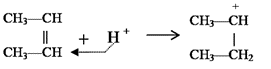
\includegraphics[]{fig1.png}
\caption{The addition of an acid proton to an olefin to produce a tert-butyl carbation}
\label{fig1}
\end{figure}

2. In the second stage, the formed carbonium ion interacts with paraffin hydrocarbon. In this case, the hydrogen anion from the tertiary carbon atom of the isoparaffin hydrocarbon passes to the carbonium ion formed at the first stage of the reaction:

\begin{figure}
\centering
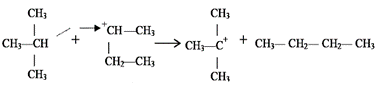
\includegraphics[]{fig2.png}
\caption{The interaction of the formed carbonium ion with paraffin hydrocarbon}
\label{fig2}
\end{figure}

3. The third stage consists in the addition of a tertiary carbonium ion to the second olefin molecule to form carbonium:

\begin{figure}
\centering
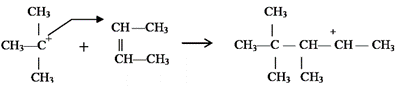
\includegraphics[]{fig3.png}
\caption{The addition of the tertiary carbonium ion to the second olefin molecule}
\label{fig3}
\end{figure}

4. The fourth stage consists in the skeletal isomerization of the secondary carbonium ion:

\begin{figure}
\centering
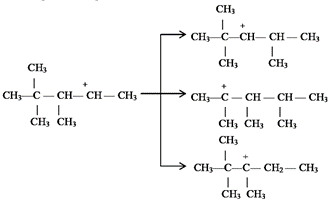
\includegraphics[height=4.3 cm]{fig4.png}
\caption{The skeletal isomerization of secondary carbonium ion}
\label{fig4}
\end{figure}

5. The fifth stage is the interaction of the formed carbonium ions with an isoparaffin molecule by a tertiary carbon-hydrogen bond with the formation of target products and a carbonium ion from isoparaffin:

\begin{figure}
\centering
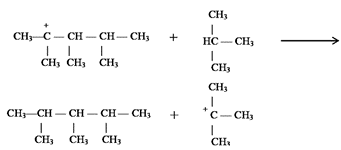
\includegraphics[height=3.5 cm]{fig5.png}
\caption{The interaction of the formed carbonium ions with the isoparaffin molecule}
\label{fig5}
\end{figure}

For ease of use when compiling the model, we will make up a chain of transformations of the sulfuric acid alkylation process (Figure 6).

\begin{figure}
\centering
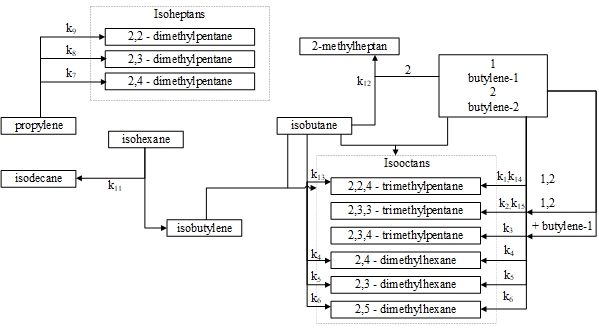
\includegraphics[height=6.5 cm]{fig6.png}
\centering
\caption{The scheme of reactions of the sulfuric acid alkylation process}
\label{fig6}
\end{figure}

It should be noted that the temperature range of the process is from 2 to 15 degrees. Determining the optimal value for a given composition of raw materials relates to the objectives of the study. In this regard, the solution of the problem of constructing a model of the process of sulfuric acid alkylation of isobutane with butylenes is relevant\cite{alkylation_mod}.

%Стыковочный абзац
Since the mathematical model of the chemical reaction is a system of differential equations, it is only possible to find the values of the constants in this system numerically (see, e.g., \cite{Gubaydullin2021}). Note that the objective function in such problems is usually multiextremal, i.e. it has many local extrema along with a global one.

%Часть ННГУ
%Numerical methods for solving such multiextremal problems (global optimization methods) differ significantly from local search methods (see, e.g., \cite{PaulaviciusZilinskas2014,Sergeyev2017}). From an algorithmic point of view, they can be divided into two classes: metaheuristic and deterministic. Metaheuristic algorithms are mainly based on the simulation of processes occurring in living nature. Typical examples of such algorithms are simulated annealing, evolution and genetic algorithms, etc. (see, e.g., \cite{Battiti2009,Eiben2015}).    Due to their relative simplicity, metaheuristic algorithms are more popular with researchers than deterministic ones.  However, the solution to a problem found by a metaheuristic algorithm is, generally speaking, local and may be well away from the global solution \cite{Kvasov2018}.

Assuming some additional properties of the objective function, it is possible to construct efficient deterministic methods for finding a global solution. For example, we can assume that the ratio of the increment of the function to the corresponding increment of the argument cannot exceed some threshold. In this case, the functions are called Lipschitzian, and the problem itself is a Lipschitz optimization problem.
This paper continues the series of papers where the parallel methods of Lipschitz optimization proposed in \cite{Strongin2000} are investigated and modified in their application to solving inverse problems of chemical kinetics.


The main part of the paper is organized as follows. Section \ref{Sec_math_mod} describes the mathematical model of the chemical reaction under study. The formal statement of the Lipschitz global optimization problem and the general scheme of search algorithms are given in Section \ref{Sec_GSA}. In this section a scheme of the proposed asynchronous parallel algorithm for solving multiextremal problems is also presented. The results of numerical solution of the inverse problem of chemical kinetics are discussed in Section \ref{Sec_Exp}.

\section{Problem Statement} \label{Sec_math_mod}

To optimize the technological process, it is necessary to know the kinetic laws and mechanism of chemical reactions, to determine which it is necessary to evaluate the kinetic parameters of chemical reactions by solving the inverse problem of chemical kinetics\cite{regularization}. In most cases, the equations of chemical kinetics are systems of ordinary nonlinear differential equations for concentrations of substances $x_{i}$ (\ref{concentration_changing}) with initial conditions (\ref{init_cond}).

\begin{equation}
  \frac{dx_{i}}{dt} = \sum_{j=1} ^J \nu_{ij} \omega_j,i=1,....I,\omega_j=k_j^0 \cdot \exp (-\frac{E_{j}}{RT})\cdot \prod_{i=1} ^M x_{i}^{|a_{ij}|}
\label{concentration_changing}
\end{equation}

\begin{equation}
t=0, x_i(0)=x_i^0,
\label{init_cond}
\end{equation}

moreover, $k_j^0 \cdot \exp (-\frac{E_{j}}{RT})$ they are called the rate constants of the reaction stages, where $I$ is the number of substances involved in the reaction; $J$ is the number of reaction stages; $v_{ij}$ are stoichiometric coefficients; $E_j$ are the activation energies of reactions, cal/mol; $R$ is the universal gas constant, cal /(mol $\cdot$ K); $T$ – temperature, K; $a_{ij}$ – stoichiometric coefficients $k_j^0$ – pre-exponential multipliers.

The inverse problem of chemical kinetics is a global optimization problem, implying the need to determine the vector of reaction rate constants ($k_1, k_2, ..., k_J$), at which the deviation of the calculated concentrations of the reaction components from the experimental ones will be minimal.
Thus, in order to determine the rate constants of the reaction, it is necessary to solve the inverse problem of chemical kinetics by repeatedly solving the direct problem – by iterating over the rate constants of the stages (or a set of pre-exponents and activation energies) according to some algorithm. To solve the optimization problem, it is necessary to minimize the functional  (\ref{functional}) deviation of experimental data from the calculated ones:

\begin{equation}
FF = \sum_{i=1} ^M \sum_{j=1} ^N |x_{ij}^{calc} - x_{ij}^{exp}|,
\label{functional}
\end{equation}
where $x_{ij}^{calc}$ are calculated values; $x_{ij}^{exp}$ are experimental data; $M$ is the number of experimental points; $N$ is the number of substances involved in the reaction.
To solve the instability problem of optimization problem (\ref{functional}), consider the minimization problem in general form

\begin{equation}
f(z) \rightarrow \inf, z \in D,
\label{problem}
\end{equation}
where $D$ is some given set, and $f: D \rightarrow R^1$ is the function (functional) specified on it. 

In this inverse problem of chemical kinetics, a number of kinetic parameters act as a point $z$ (as a rule, a vector of reaction rate constants), while the function $f$ is the deviation of the calculated concentrations of reaction components from empirical data (functional (\ref{functional})).
Problem (\ref{problem}) can be attributed to one of two classes of problems, which in the literature are called correctly posed and incorrectly posed minimization tasks, respectively. Inverse problems of chemical kinetics are incorrectly posed problems. According to Hadamard, a problem is considered to be posed correctly if 1) its solution exists, 2) the solution is unique, 3) the solution is stable to variations in the initial data. If at least one of the listed requirements is not met, the task is considered incorrectly set. The inverse problems of chemical kinetics encountered in practice usually have a solution and condition 1 is thus met. However, conditions 2 and 3 are most often not met\cite{regularization}.
For the approximate solution of ill-posed problems, special methods are required that make it possible to reliably construct a solution to problem (\ref{problem}). Such methods exist and are commonly called regularization methods. In this paper, the regularization method of A.N. Tikhonov, or the stabilization method, is used, and the classical machine learning apparatus is used – normalization of features and scaling.
The main task that we will consider will be the task of minimizing

\begin{equation}
f^0(z) \rightarrow \inf, z \in D \subset Z,
\label{minimization_problem}
\end{equation}
in which we consider the set $D$ to be a convex and closed set of Hilbert space $Z$. The function $f^0:D \rightarrow R^1$ will be considered continuous and convex on $D$. Suppose that problem (\ref{minimization_problem}) has a solution, i.e. the set $D^*$ is nonempty and denote by $z^0$ the norm-minimal solution of this problem. Suppose that instead of an exact function $f$, we know its approximation $f_{\delta},$ $\delta \in [0, \delta_0], \delta_0>0$ which is some sufficiently small number, and

\begin{equation}
|f^\delta(z) - f^0(z)| \leq \delta (1+||z||^2),  \forall z \in D. 
\end{equation}

The main construction of the Tikhonov method is the smoothing function or Tikhonov function

\begin{equation}\label{formula_T}
T_\alpha^\delta(z) \equiv f^\delta(z) + \alpha ||z||^2, z \in D.
\end{equation}
where $\alpha > 0$ is the regularization parameter. The term $\alpha||z||^2$ is called the stabilizing term. Consider the auxiliary minimization problem

\begin{equation}
T_\alpha^\delta(z) \rightarrow \inf, z \in D. 
\label{tikhonov_F}
\end{equation}

Various numerical methods can be used to approximate the solution of this problem. Suppose that as a result of a finite number of iterations we get a point $z_\alpha^{\delta,\epsilon}$ such that

\begin{equation}
T_\alpha^\delta(z) \equiv \min T_{\alpha}^{\delta}(z) \leq T_{\alpha}^{\delta} (z_{\alpha}^{\delta,\varepsilon}) \leq T_{\alpha}^{\delta} + \varepsilon,
\end{equation}
where the value $\varepsilon > 0$ characterizes the accuracy of solving the minimization problem (\ref{tikhonov_F}).In this case, the minimization problem (\ref{tikhonov_F}) for each fixed pair $\delta, \alpha$ has, as a rule, a much larger ``margin of stability'' than the original problem (\ref{problem}) and in most cases is correctly posed.

\section{Parallel Global Optimization Algorithm}\label{Sec_GSA}

\subsection{Optimization Problem}\label{Sec_GO_Problem}

As it was mentioned above, the problem of identifying the model parameter values can be considered a Lipschitz global optimization problem. From the formal point of view this problem is a mathematical programming problem of the form
\begin{equation} \label{problemN}
 \varphi^* = \varphi(y^\ast)=\min{\left\{\varphi(y):y\in D\right\}},
 \end{equation}
\begin{equation} \label{D}
 D=\left\{y\in R^N: a_i\leq y_i \leq b_i, \;  1\leq i \leq N\right\},
 \end{equation}
where the vectors $a,b\in R^N$ correspond to the lower and upper bounds of the search region and $\varphi(y)$ is the objective function which satisfies the Lipschitz condition
\begin{equation}\label{Lip}
\left|\varphi(y_1)-\varphi(y_2)\right|\leq L\left\|y_1-y_2\right\|,\; y_1,y_2 \in D.
\end{equation}


We suppose, that the function $\varphi(y)$ is multiextremal and is given as a ``black box'' (i.e. as some subroutine with a vector of parameters as its input and the calculated value of the function as its output). Moreover, it is assumed that each application of this procedure (hereinafter referred to as search trial) is a time-consuming operation. This formulation of the problem is fully consistent with the inverse problem of chemical kinetics.

There are several algorithms that can be applied to solve Lipschitz optimization problems. These include, among others, the non-uniform covering method \cite{Evtushenko2009,Evtushenko2013}, diagonal and simplicial partitions methods \cite{Zilinskas2010,Paulavicius2011}. In this paper, we used the global search algorithm proposed by Strongin \cite{Strongin2000}. Under this approach, the original multidimensional problem (\ref{problemN}) is reduced to a one-dimensional optimization problem using Peano-Hilbert curves.

In fact, using a continuous one-to-one mapping (Peano curve) $y(x)$ of the segment $[0,1]$ of the real axis onto the hyperinterval $D$ from (\ref{D}), we can reduce the original problem (\ref{problemN}) to a one-dimensional problem
\[
\varphi(y^\ast)=\varphi(y(x^\ast))=\min{\left\{\varphi(y(x)): x\in[0,1]\right\}},
\]
where the one-dimensional function $\varphi(y(x))$ will satisfy a H{\"o}lder condition
\[
\left|\varphi(y(x_1))-\varphi(y(x_2))\right|\leq H\left|x_1-x_2\right|^{1/N}
\]
with $ H=2 L \sqrt{N+3}$.
The numerical construction of various approximations of such mappings is discussed in \cite{Sergeyev2013,Strongin2000}.

Thus, the search trial at some point $x'\in[0,1]$ will involve first the image construction $y'=y(x')$, and only then the function value computation $ z' = \varphi(y')$.

\subsection{Characteristic Algorithms}

%Характеристический алгоритм
The global search algorithm we used belongs to the class of characteristic algorithms, which greatly simplifies the process of its parallelization. Recall that a numerical optimization method belongs to the class of characteristic algorithms if the algorithmic scheme of this method can be described as follows.

At the first iteration the trials are performed at the points $x^1 = 0$ and $x^2 = 1$. Then any next $(k+1)$, $k \geq 2$, iteration of global search is executed in the following way.

\begin{enumerate}
	\item 
Renumber points of the previous trials by increasing their $x$-coordinates (the new order is marked with subscript)
\[
0=x_0<x_2<...<x_{k}=1.
\]

	\item 
Calculate for every interval $(x_{i-1},x_i), 1\leq i\leq k$, a value $R(i)$ called \textit{the interval characteristic}. In the general case, $R(i)$ can depend on the points $x^i$ and the trial results $z^i=f(x^i), 1 \leq i \leq k$.

	\item 
Find the interval $(x_{t-1},x_t)$ which has the largest characteristic $R(t)$, i.e.
\[
R(t) = \max \left\{ R(i): \; 1\leq i\leq k \right\}.
\]

	\item 
Examine the stop condition
\[
\Delta_t \leq \epsilon ,
\]
where $\epsilon>0$ is a given accuracy. If the stop condition is satisfied, then the global search has to be terminated; otherwise the calculations should continue.

	\item 
Select a point $x^{k+1}$ of the current iteration within the interval $(x_{t-1},x_t)$ in accordance with some rule $S(t)$, i.e.
\[
x^{k+1} = S(t)\in(x_{t-1},x_t).
\]
	
	\item 
Calculate the function value $z^{k+1} = f(x^{k+1})$.

	\item 
Evaluate a global minimum estimate. 

	\item 
Increase the iteration number $k=k+1$ and proceed to the next iteration.
\end{enumerate}


As a possible interpretation of this scheme, we can consider an interval characteristic $R(i)$ as a measure of the global minimum being within the interval
$(x_{i-1},x_i)$.
To construct a concrete form of the interval characteristic, we can use a lower envelope (or minorant) of the function to be minimized or a mathematical expectation of function values, etc. 
Most well-known global optimization methods can be formulated in accordance with this characteristic scheme, e.g.,
\begin{itemize}
\item a uniform grid method with a successively reduced step;
\item a random search (Monte-Carlo) algorithm;
\item the Piyavskii algorithm \cite{Piyavskii1972};
\item one-step bayesian algorithms proposed by Kushner and {\v Z}ilinskas \cite{Zilinskas1989};
\item information algorithms proposed by Strongin \cite{Strongin2000}.
\end{itemize}
All these methods are based on different mathematical models but are presented in the general characteristic scheme.

It should be also noted that the length of the interval with the largest characteristic is examined at the stop condition.
It is possible if the optimization method converges to the global minimum.
Details of these methods are given in the sources cited. %Здесь же отметим основные моменты
Here we highlight the main points.

For the Piyavskii method the interval characteristic $R(i)$ is an estimate (with the inverse sign) of the least value of the objective function $f(x)$ within the
interval $(x_{i-1},x_i)$. As a result, the point of a new trial is taken within the interval containing the estimate of the least value of $f(x)$ over the search domain.

The Kushner technique and the Zilinskas method have been constructed in the framework of the approach when the objective function is considered as
a sample of some Wiener process. For the Kushner technique the point $x^{k+1}$ of the current iteration is the most probable point at which the function value
$f(x^{k+1})$ is not greater than the value
\[
z_k^* -\gamma (z_k^+-z_k^*),
\]
where $z_k^+$ and $z_k^*$ are estimates of maximum and minimum function values respectively. For the Zilinskas method $x^{k+1}$ is the point where the maximum average improvement of the current estimate of the global extremum is expected.

The Strongin global search algorithm has been constructed in the framework of the information approach to global optimization (see \cite{Strongin2000}). This method has an adaptive scheme to evaluate a numerical estimate of the unknown Lipschitz constant.


\subsection{Parallel Algorithm with Asynchronous Trials}\label{Sec_PGSA}

As the global search algorithm (GSA) belongs to the class of characteristic algorithms, this suggests a possible way to parallelize it. 
As previously mentioned, the characteristic of the interval $R(i)$ can be regarded as some measure of finding the global minimum point in this interval. Then, instead of a single best interval, several intervals with the highest characteristics can be chosen at once and successive trials can be carried out in these intervals in parallel. Moreover, the scheme of characteristic algorithms also allows asynchronous parallelization, which minimizes downtime of processors when trial complexity depends on a particular point in the search domain. 

Now, let us examine the parallel algorithm with asynchronous trials in more detail. It implements a paralleling scheme of the ``master/worker'' type. The master process accumulates search information, evaluates on its basis the Lipschitz constant for the target function, determines new trial points and sends them to the worker processes. Worker processes receive the points from the master, carry out new trials in these points and send the results to the master.

When describing the parallel algorithm, we assume that we have $p+1$ computational processes: one master and $p$ worker processes.
 
At the beginning of the search, the master process (let it be process No. 0) initiates $p$ parallel  trials at $p$ different points of the search domain, two of which are boundary points and the rest are internal points, i.e. at the points $\{y(x^1), y(x^2), ...,y(x^p)\}$, where $x^1 = 0$, $x^p = 1$, $x^i\in(0,1), i=2,..., p-1$.

Suppose now that $k$ trials have been performed (in particular, $k$ can be 0), and the worker processes perform trials at the points $\{y(x^{k+1}), y(x^{k+2}), ...,y(x^{k+p})\}$. 

If a worker process completes the trial at some point (let it be the point $y(x^{k+1})$ corresponding to process No. 1) then it sends to the master process the results of the trial. Note that in this case we will have a set of inverse images of the trial points
\[
S_k = \left\{ x^{k+1},x^{k+2},...,x^{k+p} \right\},
\]
where the trials have already started but have not yet been completed.

Having received the trial results at the point $y(x^{k+1})$ from the worker process, the master in turn selects a new trial point $x^{k+p+1}$ for it according to the rules that correspond to the scheme of the characteristic algorithm.

\begin{enumerate}
	\item 
Renumber the set of inverse images of the trial points 
\[
X_k = \left\{x^1, x^2,...,x^{k+p} \right\},
\]
containing all inverse images at which the trials have either been carried out or are being carried out in ascending order (marked with subscript) , i.e.
\[
0=x_1<x_2<...<x_{x+p}=1.
\]
	\item
Calculate the values
\[
M_1=\max \left\{ \frac{ \left|z_i - z_{i-1} \right|}{(x_i-x_{i-1})^{1/N}} : x_{i-1} \notin S_k, x_i \notin S_k, 2\leq i\leq k+p \right\},
\]
\[
M_2=\max \left\{ \frac{ \left|z_{i+1} - z_{i-1} \right|}{(x_{i+1}-x_{i-1})^{1/N}} : x_i \in S_k, 2\leq i < k+p \right\},
\]
\[
M=\max\{M_1,M_2\},
\]
where $z_i=\varphi(y(x_i))$ for all $x_i \notin S_k$. 
%The values of $z_i$ at the points $x_i \in S_k$ are undefined, as the trials at these points have not yet been completed. 
If $M$ equals 0, then assume $M=1$.

	\item
Assign to each interval $(x_{i-1},x_i), \; x_{i-1} \notin S_k, x_i \notin S_k$, the characteristic $R(i)$, which is calculated using the formula
\begin{equation} \label{R}
R(i)=rM\Delta_i+\frac{(z_i-z_{i-1})^2}{rM\Delta_i}-2(z_i+z_{i-1}),
\end{equation}
where $r>1$ is the method parameter and $\Delta_i=\left(x_i-x_{i-1}\right)^{1/N}$.

	\item
Find the interval $[x_{t-1},x_t]$ to which the maximum characteristic corresponds, i.e.
\[
R(t) = \max \left\{ R(i): \; x_{i-1} \notin S_k, x_i \notin S_k, \; 2\leq i\leq k+p \right\}.
\]
	\item
Determine the inverse image $x^{k+p+1} \in (x_{t-1},x_t)$ of the new trial point according to the formula
\[
x^{k+p+1} = \frac{x_{t}+x_{t-1}}{2} - \mathrm{sign}(z_{t}-z_{t-1})\frac{1}{2r}\left[\frac{\left|z_{t}-z_{t-1}\right|}{M}\right]^N.
\]
\end{enumerate}

Immediately after calculating the next trial point $y^{k+p+1} = y(x^{k+p+1})$, the master process adds it to the set $S_k$ and forwards it to the worker process which initiates a trial at this point.

The master process completes the algorithm when one of two conditions is met: $\Delta_{t}<\epsilon$, $k+p>K_{max}$.
The first one corresponds to stopping the algorithm by accuracy, the second one, by the number of trials. The real number $0<\epsilon<1$ and the integer $K_{max}>0$ are the algorithm parameters.

\section{Numerical Experiments} \label{Sec_Exp}

To determine the constants of the reactions of the process, it is necessary to solve a system of differential equations describing the change in the concentration of reaction components over time \cite{cao2019}.

%


In preliminary experiments, we estimated the approximate time to calculate one objective function using the sequential algorithm. The computer architecture used for the experiments was Intel(R) Core(TM) i7-10750H CPU @ 2.60GHz 2.59 GHz. The average calculation time of the objective function was about $0.2$ sec, which characterizes the problem as being computationally complex.  Solving the problem with a sequential algorithm would require at least 1 million trials and thus at least 54 hours (as an estimate). Therefore, only a parallel algorithm with a stopping criterion based on the number of trials $K_{max}=10^6$ was used for the calculations. 

Numerical experiments were performed using the parallel asynchronous algorithm outlined in Section \ref{Sec_PGSA}, running $160$ processes: $159$ processes calculated the values of the objective function (worker processes) while $1$ master process controlled the algorithm. The Lobachevsky  supercomputer (University of Nizhni Novgorod) was used for the experiments. The asynchronous global optimization algorithm was implemented in C++ (GCC 9.5.0 and Intel MPI were used); the computation of objective function values was implemented in Python 3.9.


\begin{table}
\caption{Dependence of the function minimum value $\varphi^*$ on the regularization parameter $\alpha$}
\label{table_1}
\begin{center}
\begin{tabular}{ccc}
\hline\noalign{\smallskip}
 $\alpha$      & $\varphi^*$  & Time (sec.) \\
\hline\noalign{\smallskip}
0.0	    &	0.57392		&	838.9	\\
0.001	&	0.54075		&	853.9	\\
0.002	&	0.547907	&	850.0	\\
0.003	&	0.583529	&	831.5	\\
0.004	&	0.579725	&	821.4	\\
0.005	&	0.615638	&	815.4	\\
0.006	&	0.612614	&	834.7	\\
0.007	&	0.619546	&	807.3	\\
0.008	&	0.604817	&	830.4	\\
0.009	&	0.63001		&	814.4	\\
0.01	&	0.632944	&	825.2	\\
0.02	&	0.669092	&	155.8	\\
0.03	&	0.68152		&	809.2	\\
0.04	&	0.736035	&	816.4	\\
0.05	&	0.729415	&	804.7	\\
0.07	&	0.759134	&	803.6 \\
0.06	&	0.723404	&	810.9	\\
0.08	&	0.808238	&	811.8	\\
0.09	&	0.837868	&	828.6 \\
0.1		&	0.810454	&	806.2	\\
\noalign{\smallskip}\hline
\end{tabular}\end{center}\end{table}

%Ускорение составило примерно $230$ раз.
The short time for solving the problem when using the parallel algorithm (approximately 14 minutes for 1 problem) allowed a thorough investigation of the dependence of the solution on the regularisation parameter $\alpha$. Table \ref{table_1} shows the minimum values of the objective function found for the corresponding value of the regularization parameter and the time for solving the problem (in seconds).
%and the time speedup in comparison to the estimated problem solution time when using the sequential method. 
The method parameter $r=4.0$ from (\ref{R}) and the accuracy $\epsilon = 10^{-4}\left\|b-a\right\|$ were used in the runs. After a given number of iterations or after reaching the specified accuracy with the global search method, the solution was refined by the Hooke-Jeeves local method \cite{HookJeeves} with an accuracy of $\epsilon = 10^{-4}\left\|b-a\right\|$.

A detailed study of the region of the regularization parameter values in the neighborhood of $\alpha$ equal to zero (from $0.1$ to $0.01$ in steps of $0.01$ and from $0.01$ to $0.001$ in steps of $0.001$) revealed that the value of the minimum decreases with decreasing $\alpha$. The best solution of $0.54075$ was obtained with the regularisation parameter $\alpha = 0.001$.

In the course of the research, the functional $f(z)$ was calculated without taking into account the addition of the regularization term (figure \ref{fig7}). Then a similar calculation was carried out taking into account the regularization term. The results for $\alpha=0.002$ is $0.527$ with regularization, and $0.547$, respectively.

\begin{figure}
\centering
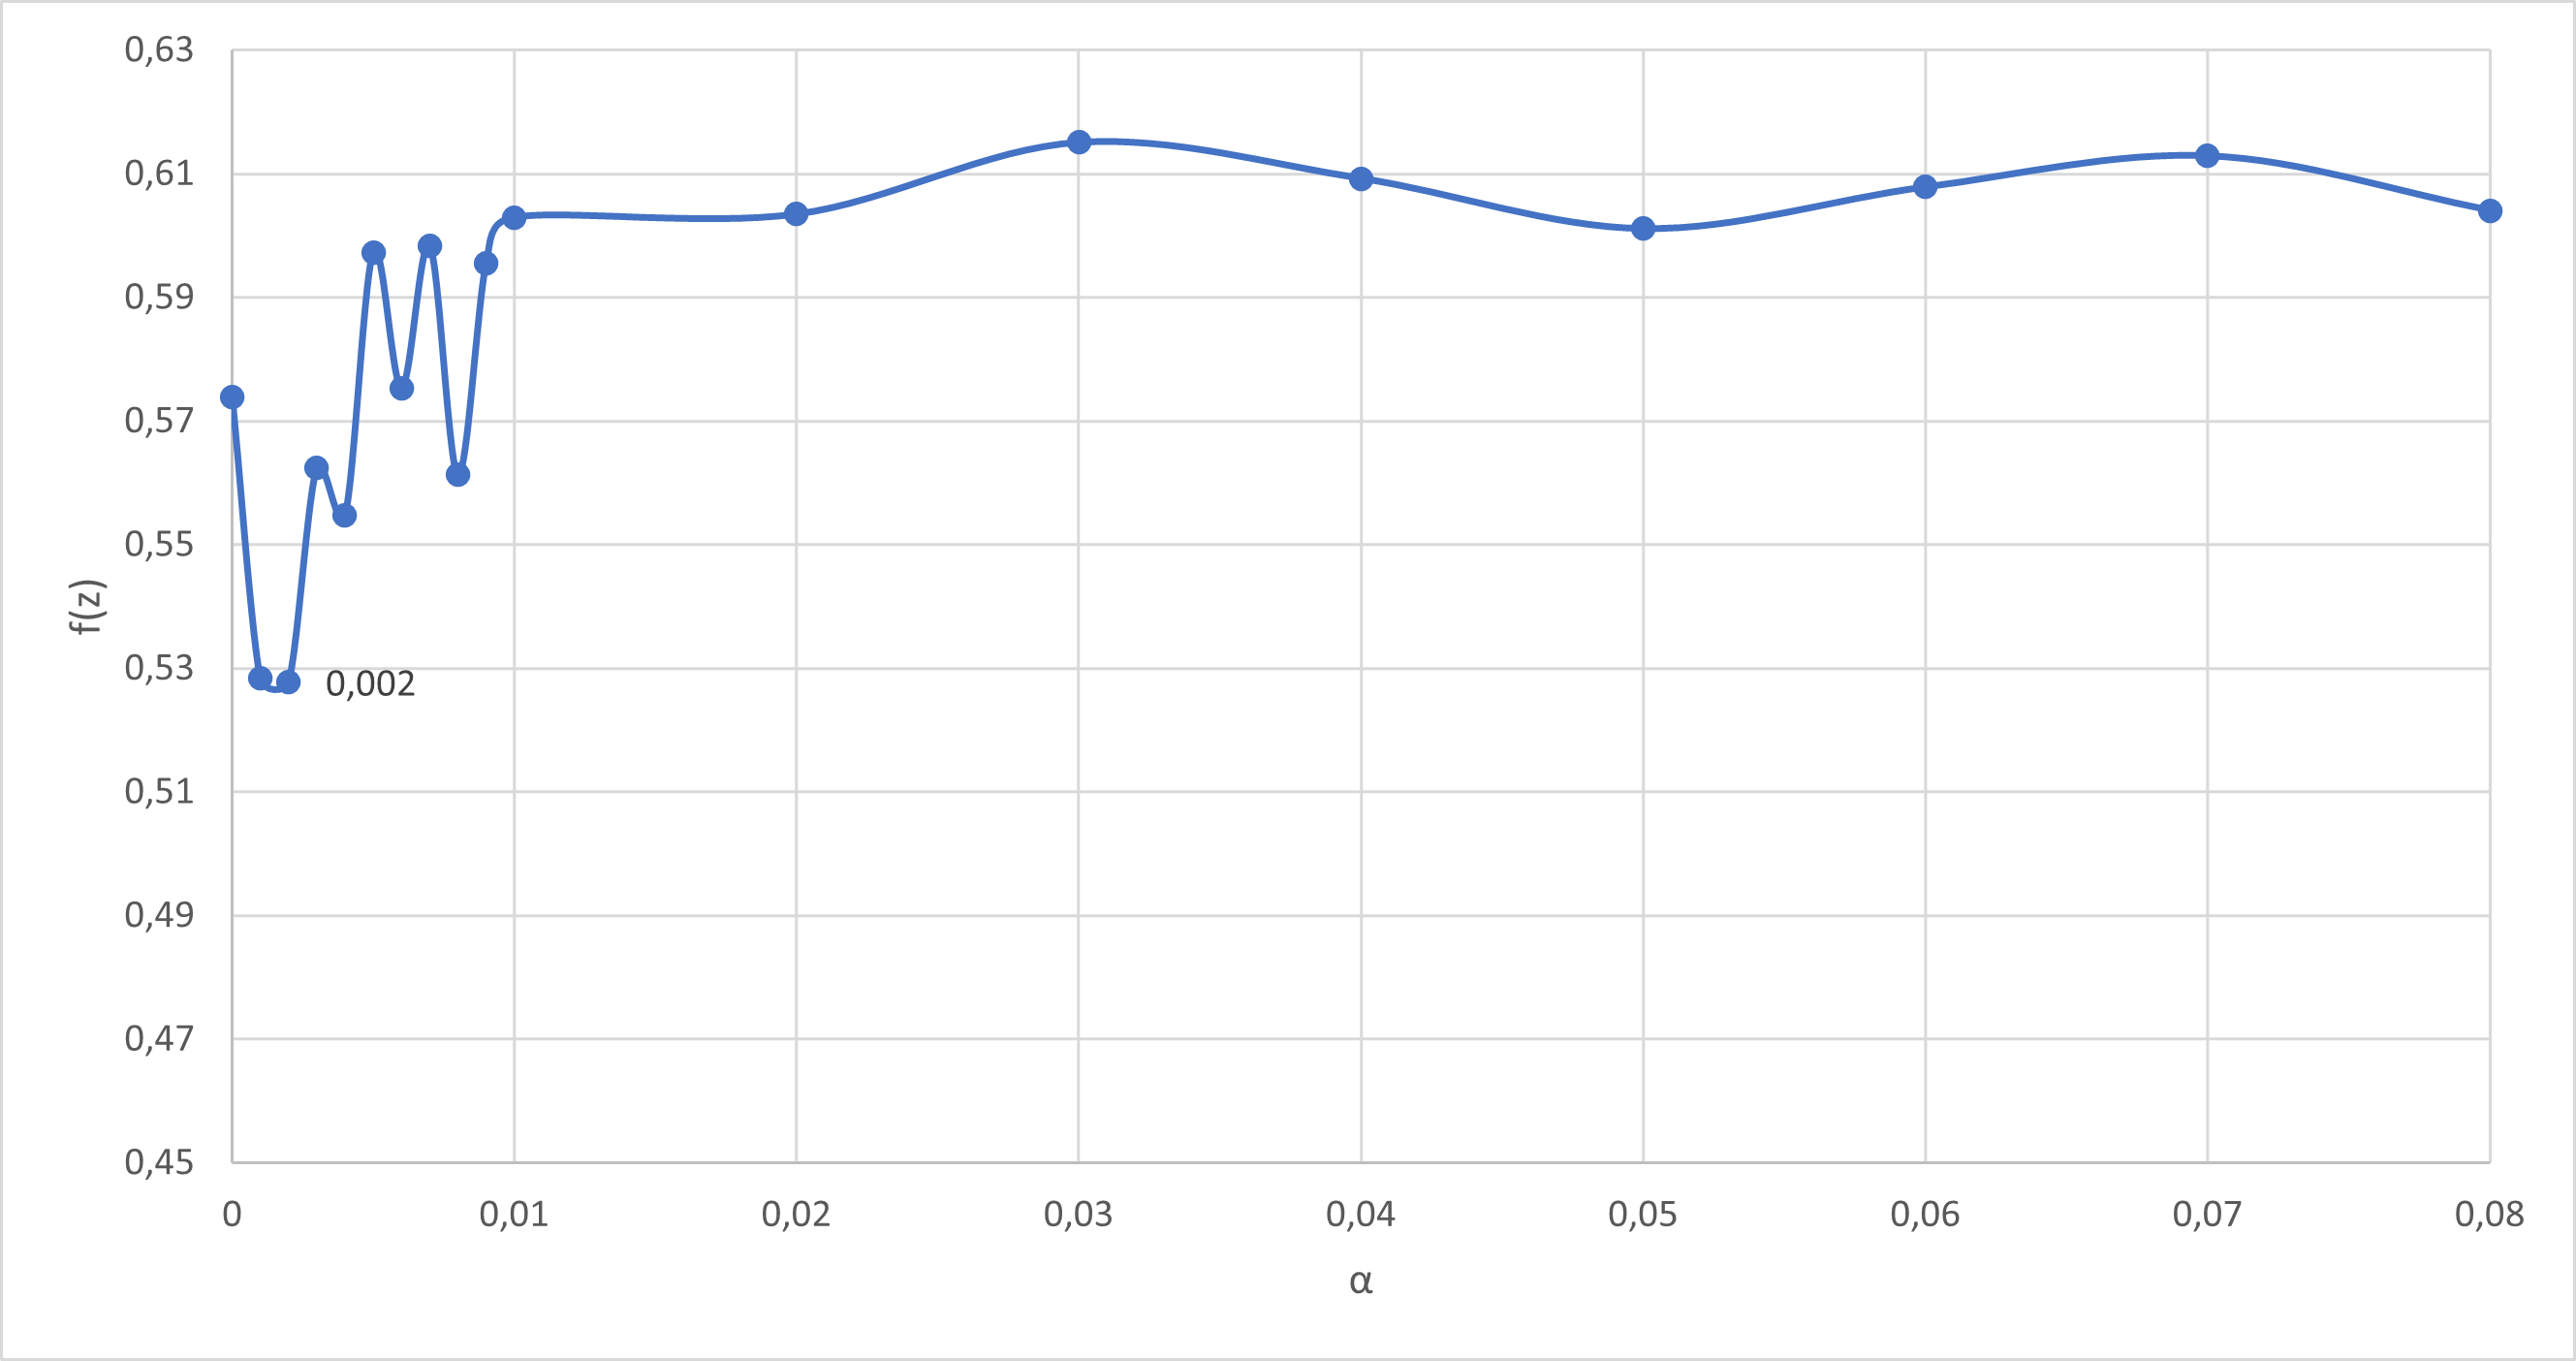
\includegraphics[height=6.0 cm]{fig7.png}
\caption{The value of the functional $f(z)$ without taking into account the addition of the regularization term}
\label{fig7}
\end{figure}

The speedup of the parallel global optimization algorithm was estimated for the problem in which the best solution was found, i.e. the problem with regularization parameter $\alpha = 0.001$.
Since solving the problem in serial mode would require about two days, the acceleration was evaluated in relation to a parallel launch involving a smaller number of processes.
Table \ref{table_2} shows running time and acceleration of the parallel algorithm using 80 and 160 processes in relation to running time using 40 processes

\begin{table}
\caption{Speedup of the parallel  global optimization algorithm}
\label{table_2}
\begin{center}
\begin{tabular}{ccc}
\hline\noalign{\smallskip}
 $p$     & Time (sec.)  & Speedup \\
\hline\noalign{\smallskip}
40	&	2778.7		&	---	\\
80	&	1495.5		&	1.9	\\
160	&	853.9	    &	3.3	\\
\noalign{\smallskip}\hline
\end{tabular}\end{center}\end{table}



\section{Conclusion} 

Thus, in this article an incorrect problem was solved using the Tikhonov regularization method and the reaction constants of the process of sulfuric acid alkylation of isoalkanes by alkenes were found. Defined fun the optimization method allowed us to find a fairly accurate description of the experimental data. The Tikhonov regularization method considered by the authors is planned to be used in the future to build kinetic models of other chemical processes.

The use of the parallel global search algorithm showed good results. The solution of the problem was obtained at about 15 minutes using the Lobachevsky supercomputer, while the estimated time for solving the problem with a sequential algorithm would be more than 50 hours. When conducting the experiments 160 processes on the supercomputer nodes were involved in the calculations. However, an increase in the dimension of the global optimization problem being solved (for complex inverse problems of chemical kinetics the number of parameters can be hundreds) will lead to a decrease in the quality of the search.

A possible direction for further research is the development of methods for analyzing the accumulated search information in order to identify groups of parameters that have slight effect on the objective function. To find the optimal values of such parameters, it is sufficient to use local optimization methods. Such an analysis can be carried out, for example, using machine learning methods. In this case, the cost of solving the problem as a whole will decrease, and it will be possible to obtain a global solution with good accuracy in an acceptable time.


\medskip

\textbf{Acknowledgments}. This study was supported by the Ministry of Science and Higher Education of the Russian Federation (project no. FSWR-2023-0034), and by the Research and Education Mathematical Center (project no.  075-02-2022-883). This research was partially funded by the state task of the Institute of Petrochemistry and Catalysis of the Russian Academy of Sciences (theme No. FMRS-2022-0078).

%This research was partially funded by the Ministry of Science and Higher Education of the Russian Federation, project no. FSWR-2023-0034, by the Research and Education Mathematical Center, project no. 075-02-2022-883 (development of the parallel global optimization algorithm), and by the Ministry of Science and Higher Education of the Russian Federation, project no. FMRS-2022-0078 (investigation of chemical kinetics problem).


%
% ---- Bibliography ----
%
\bibliographystyle{spmpsci}
\bibliography{example-bibtex}{}

\end{document}
